\documentclass[11pt,spanish,a4paper,openany,notitlepage]{article}
%-------------------------------------Paquetes------------------------------------------------------
\usepackage[spanish]{babel}  	% Traduce los textos a castellano
\usepackage[utf8]{inputenc}	% Permite escribir directamente áéíóúñ
\usepackage{t1enc}            	% Agrega caracteres extendidos al font
\usepackage{amsmath} 		%Permite imprimir mas opcciones matematicas
\usepackage{graphicx}		%Permite agregar imagenes al informe
\usepackage{multicol}  		%Permite dividir el texto en varias columnas
\usepackage{anysize}		%Permite modificar los margenes del documento
\usepackage{float} 		%Permite utilizar H para colocar las imagenes en un lugar especifico 
\usepackage{multirow}		%Permite dividir las tablas en subtablas
\usepackage{booktabs}		%Permiten manejar mejor el tamaño de las tablas
\usepackage{tabulary}		%Permiten manejar mejor el tamaño de las tablas
%---------------------------------------------------------------------------------------------------

%---------------------------------------Configuraciones de pagina-----------------------------------
\marginsize{2.5cm}{2.5cm}{1cm}{1cm}
%---------------------------------------------------------------------------------------------------

%---------------------------------------Definiciones propias----------------------------------------
\newcommand{\grad}{\hspace{-2mm}$\phantom{a}^{\circ}$} %El º que no existe como comando
%---------------------------------------------------------------------------------------------------

\begin{document}

\setcounter{page}{0}

\begin{center}
\textbf{\LARGE U.B.A.    FACULTAD DE INGENIERÍA\\
$\phantom{a}$\\
Departamento de Computación\\
$\phantom{a}$\\
Técnicas de programación concurrente I  75-59\\
Informática\\
$\phantom{a}$\\
TRABAJO PRÁCTICO N\grad 1\\
$\phantom{a}$\\
\textit{ConcuDelivery}}

\end{center}
$\phantom{a}$\\
Curso 2015 - 1er Cuatrimestre\\
\phantom{a}\\

\begin{tabular}{| l l |  r}%Datos de los integrantes del grupo
\hline
\multicolumn{3}{|c|}{Grupo N\grad 7}\\
\hline
\multicolumn{2}{|c|}{APELLIDO , Nombres} &\multicolumn{1}{c|}{N\grad  Padrón}\\
\hline
MARTIN & Debora Elisa & \multicolumn{1}{c|}{90934}\\ \hline
MARTINEZ & Gaston Alberto & \multicolumn{1}{c|}{91383}\\ \hline
MERLO SCHURMANN  & Bruno Javier  & \multicolumn{1}{c|}{91818}\\ \hline
\end{tabular}
\\

\phantom{X\\X\\X\\X\\X\\}
\begin{tabular}{|l|}%Datos de los integrantes del grupo
\hline
Observaciones: \\
\phantom{XXXXXXXXXXXXXXXXXXXXXXXXXXXXXXXXXXXXXXXXXXXXXXX}\\
\phantom{XXXXXXXXXXXXXXXXXXXXXXXXXXXXXXXXXXXXXXXXXXXXXXX}\\
\phantom{XXXXXXXXXXXXXXXXXXXXXXXXXXXXXXXXXXXXXXXXXXXXXXX}\\
\phantom{XXXXXXXXXXXXXXXXXXXXXXXXXXXXXXXXXXXXXXXXXXXXXXX}\\
\phantom{XXXXXXXXXXXXXXXXXXXXXXXXXXXXXXXXXXXXXXXXXXXXXXX}\\
\phantom{XXXXXXXXXXXXXXXXXXXXXXXXXXXXXXXXXXXXXXXXXXXXXXX}\\
\phantom{XXXXXXXXXXXXXXXXXXXXXXXXXXXXXXXXXXXXXXXXXXXXXXX}\\
\phantom{XXXXXXXXXXXXXXXXXXXXXXXXXXXXXXXXXXXXXXXXXXXXXXX}\\
\hline
\end{tabular}

\newpage
\tableofcontents
\newpage

\section{Análisis del problema}

El problema consiste en realizar la simulación del funcionamiento de un delivery de pizza. La misma 
empieza con la toma de los pedidos, luego el amasado y preparado de las pizzas, la cocción de 
éstas, y por último la entrega y cobro. Además, una supervisora realiza un control de la caja 
registradora periódicamente.

Mientras sea el horario de atención, las telefonistas tomarán los pedidos, siendo éstos de solo una 
pizza por cada uno. Los pedidos son pasados a las cocineras, quienes prepararán la pizza y la 
pondrán a cocinar en un horno por un tiempo predeterminado. Cuando finaliza la cocción, las cadetas 
son las encargadas de retirar las mismas, realizar la entrega y depositar el dinero en la caja. 
Además, solo se toman pedidos mientras que la cantidad de pendientes no supere el doble de la 
cantidad de cocineras, para no sobrecargarlas de trabajo. 
Cuando el horario de atención finaliza, se dejan de atender pedidos. Se procesan y entregan los que 
ya estaban tomados, y se cierra el delivery.
La supervisora revisará periódicamente la caja mientras la pizzería esté abierta, siempre no esté 
siendo usada por una cadeta.

La cantidad de telefonistas, cocineras, hornos y cadetas, y el intervalo de tiempo entre una 
revisión de caja y la siguiente, están determinados en un archivo de configuración.

\newpage

\section{División del proyecto en procesos}

Luego de analizar el problema y los requerimientos del mismo, se decidió dividir el programa en 
cinco procesos principales: uno por cada sección de la pizzería (recepción de pedidos, cocina, 
hornos y entregas) y uno para la supervisión de la caja. Cada uno de estos lanzará subprocesos para 
procesar las tareas de forma atómica, representando a una entidad de esa sección que la realiza. 
Por ejemplo, en el proceso que representa la cocina, se lanzan subprocesos para preparar los 
pedidos y enviarlos a los hornos, que representan a una cocinera amasando y poniendo las pizza a 
cocinar.
Un proceso principal se encargará de la inicialización del ambiente, y el control de los cinco 
procesos principales

\section{Comunicación entre procesos}

Los procesos que representan a las partes de la pizzeria deben comunicarse entre ellos, cada una 
con la sección anterior y la posterior. Por lo tanto, las relaciones son las siguientes:

\begin{center}
\begin{tabular}{|c|c|}
\hline
Sección & Se comunica con \\
\hline
Recepción & Cocina \\
\hline
Cocina & Recepción y Hornos \\
\hline
Hornos & Cocina y Entregas \\
\hline
Entregas & Hornos \\
\hline
\end{tabular}
\end{center}

Además de las anteriores, el programa principal es el punto de entrada del sistema, por lo que debe 
redirigir los pedidos que se ingresen al proceso de la Recepción. 

Por último, la supervisora y cada cadeta deben acceder a la caja de a una por vez. Por lo tanto, 
deben coordinarse para no usar la registradora más de una al mismo tiempo.

\subsection{Comunicación Programa Principal-Recepción}

Los pedidos se ingresan por entrada estandar, por lo que estos dos procesos deben comunicarse de 
forma que todo lo ingresado en el programa principal sea edirigido a la Recepción. 

\subsection{Comunicación Recepción-Cocina}

La recepción y la cocina deben comunicarse para pasar los pedidos tomados por las telefonistas a 
las cocineras. Además, la recepción debe saber cuando se llegó a la cantidad de pedidos pendientes 
máxima para no tomar nuevos hasta que alguno sea atendido.

\subsection{Comunicación Cocina-Hornos}

La cocina y los hornos deben comunicarse de manera que las cocineras puedan colocar un pedido 
procesado a cocinarse. Deben saber si hay algún horno libre para poder hacerlo, caso contrario 
deben esperar a que alguno se libere.

\subsection{Comunicación Hornos-Entregas}

En cuanto a la comunicación entre los hornos y la sección de entregas, debe permitir que una cadeta 
sea notificada cuando termina la cocción en un horno, para retirar el pedido del mismo y realizar 
la entrega. Además, al momento de cerrar, las cadetas necesitan saber cuando ya no quedan hornos 
ocupados para poder dar por terminada su actividad (dado que deben procesarse y entregarse todos 
los pedidos pendientes al cerrar).

\subsection{Comunicación Entregas-Supervisora}

Entre las cadetas de la sección de entregas y la supervisora deben notificarse mutuamente cuando la 
caja está siendo utilizada, ya que solo una persona puede acceder a la misma. 

\section{Mecanismos de concurrencia utilizados}

Se han utilizado, para cada caso descripto anteriormente, los siguientes mecanismos de concurrencia:

\subsection{Comunicación Programa Principal-Recepción}

Se utiliza un unnamed pipe para enviar los pedidos ingresados por entrada estandar en el programa 
principal (writer) a la recepción (reader). Se opto por este mecanismo dado que se pretende conectar un proceso padre con un proceso hijo.\\ 
Se utilizo un lock para proteger al pipe. El uso de un lock evita que se cierre el pipe cuando todavía quedan pedidos pendientes encolados. El lock se pide al
crear el objeto que simula la recepcion (en el proceso hijo) y no se libera hasta que no queden pedidos pendientes. En el proceso padre, el lock se pide al momento de intentar cerrar y liberar el pipe.

\subsection{Comunicación Recepción-Cocina}

Se utiliza una FIFO para enviar los pedidos desde las recepcionistas hacia la cocina. En funcionamiento es similar al pipe que conecta el programa principal, pero debido a que no son procesos con una relacion padre-hijo, no se podia utilizar un pipe.\\
Al igual que para el pipe, se utilizo un lock para evitar cerrarla antes que este vacia. Se comporta de la misma manera que el anteriormente mencionado.

\subsection{Comunicación Programa Principal-Cocina}

El programa principal debe tener alguna manera de poder monitorear la cantidad de pedidos que se pueden seguir aceptando. Se puede seguir tomando pedidos mientras que el numero de pedidos tomados menos el de pedidos procesados por la cocina, no supere al doble del numero de cocineras.\\
Se opto para esto, utilizar un semaforo compartido entre ambos. El semaforo se inicializa en el doble del numero de cocineras. Al recibir un pedido por consola, el programa principal decremetan este semaforo; mientras que en la cocina se aumenta al aceptar un pedido. 

\subsection{Comunicación Cocina-Hornos}

\subsection{Comunicación Hornos-Entregas}

\subsection{Comunicación Entregas-Supervisora}

\newpage

\section{Diagrama de procesos}

\begin{figure}[h]
\begin{center}
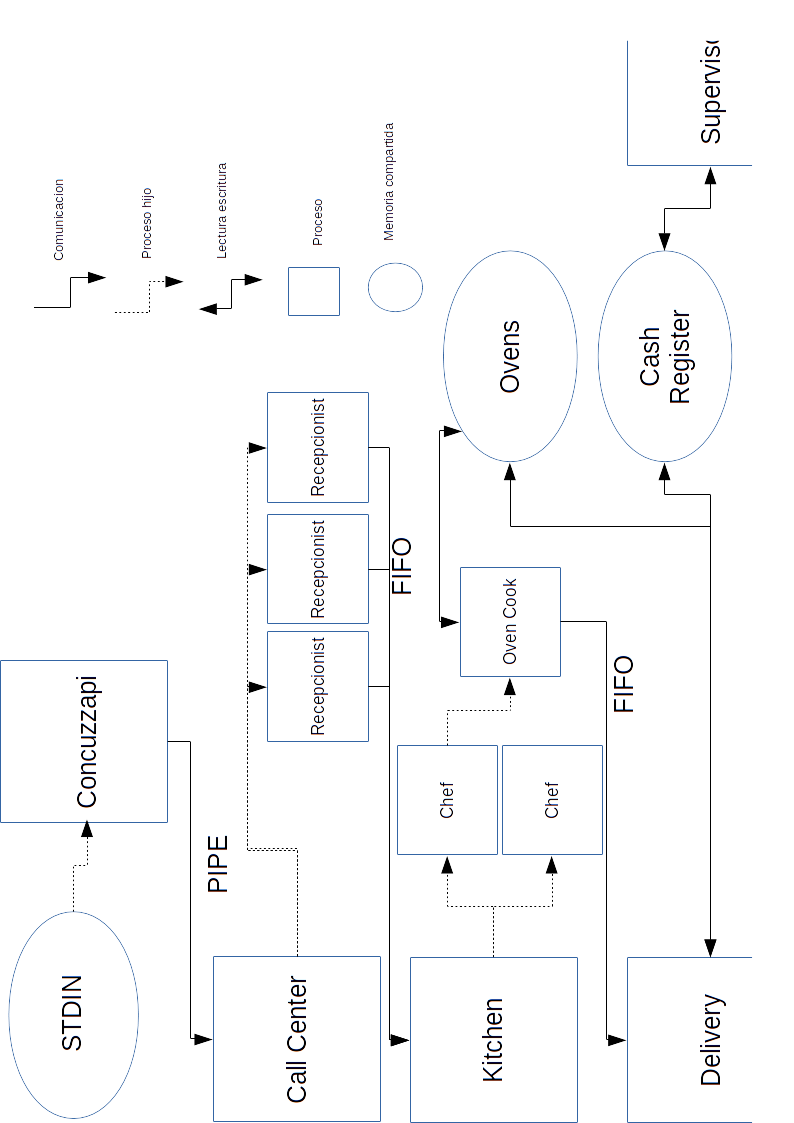
\includegraphics[width=250pt]{./informe/Modelo-de-procesos.png}
\caption{Diagrama de procesos}
\end{center}
\end{figure}

\newpage

\section{Diagrama de clases}

\begin{figure}[h]
\begin{center}
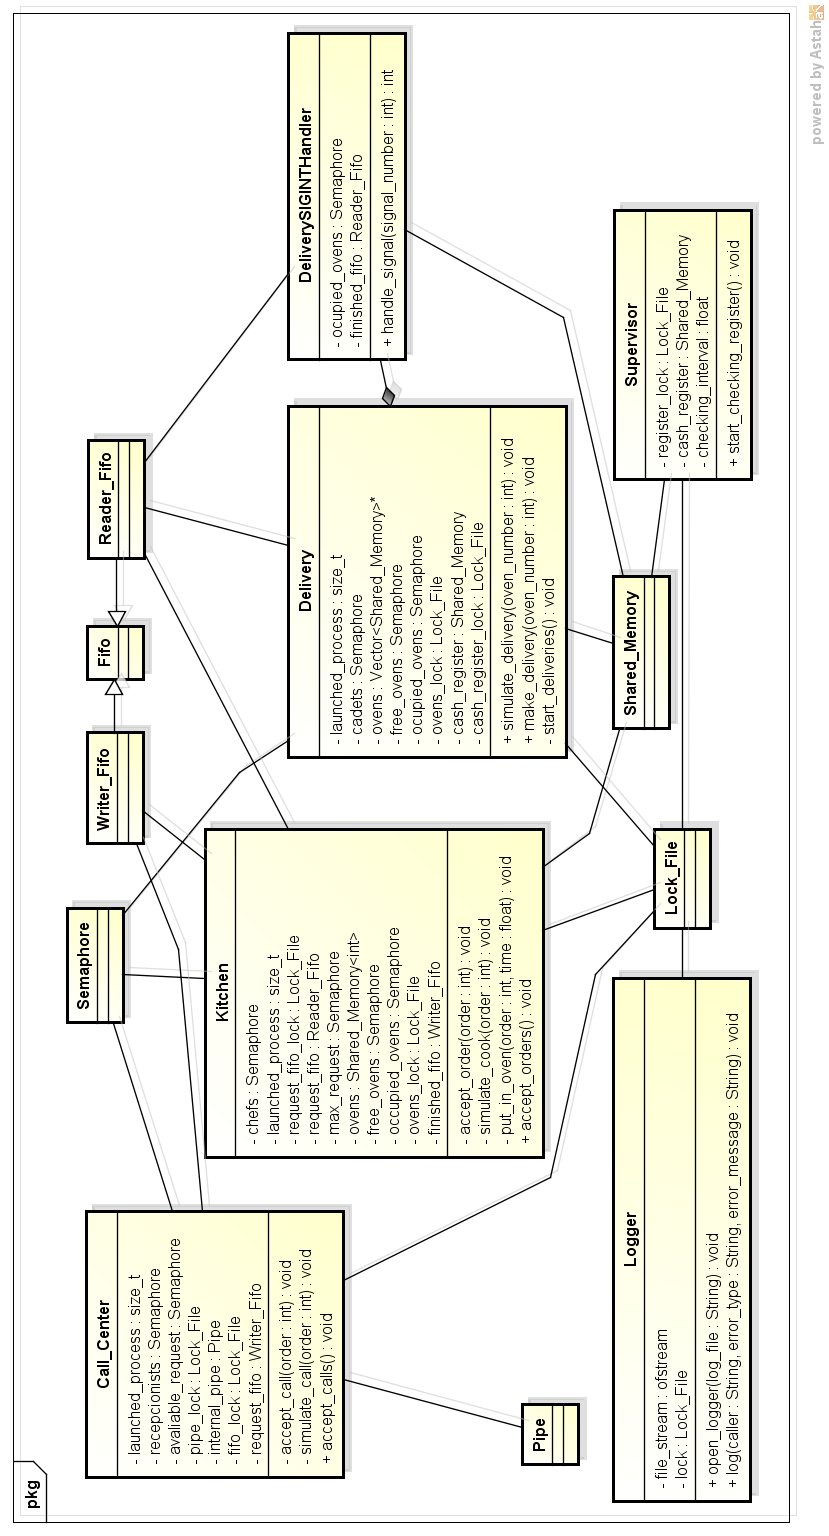
\includegraphics[width=250pt]{./informe/diagrama-clases.png}
\caption{Diagrama de clases}
\end{center}
\end{figure}

\newpage

\section{Diagrama de transición de estados}

\begin{figure}[h]
\begin{center}
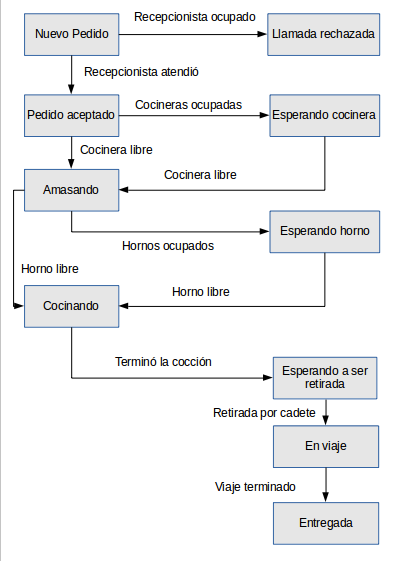
\includegraphics[width=250pt]{./informe/diagrama-estados-pizza.png}
\caption{Diagrama de transición de estados}
\end{center}
\end{figure}

\end{document}
